\documentclass[11pt,letterpaper]{article}
\usepackage[margin=1in,top=0.85in,bottom=0.87in,footskip=0.44in]{geometry}
\usepackage{amsmath,amssymb,amsthm,graphicx,booktabs,xcolor}
\definecolor{linkblue}{HTML}{15545B}
\usepackage[colorlinks=true,linkcolor=linkblue,citecolor=linkblue,urlcolor=linkblue,
            pdftitle={Information encoded in relative boosts at a gravitational corner},
            pdfauthor={Pioneer research manuscript}]{hyperref}
\newtheorem{theorem}{Theorem}
\newtheorem{lemma}[theorem]{Lemma}
\newcommand{\Tr}{\operatorname{Tr}}
\newcommand{\dd}{\mathop{}\!{\rm d}}
\newcommand{\E}{\mathbb E}
\newcommand{\sg}{s_*}
\newcommand{\Prob}{P^{\mathrm{opt}}}
\renewcommand{\arraystretch}{1.15}
\setlength{\emergencystretch}{1.2em}
\raggedbottom

\begin{document}
\begin{center}
{\small\scshape Pioneer \enspace / \enspace Theoretical physics}\par
\vspace{0.65em}
{\LARGE\bfseries Information encoded in relative boosts\\[2pt]
at a gravitational corner}\par
\vspace{0.5em}
{\small 26 November 2026}
\end{center}

\begin{abstract}
How small a change of relative frame can two gravitational boundaries distinguish in a single preparation? We take as inputs the area-generated boost and the limiting area distribution of a clock-bounded Schwarzschild causal diamond. A coherent acceptance filter acts on area, and an integer multiple of a real boost encodes the message. For fixed alphabet size $M$, nonvanishing preparation probability and exact orthogonality in all sufficiently large finite diamonds are possible precisely when $\eta\sg>4\pi^2(1-1/M)$, where $\sg$ is the area bound in units of $4G_N\hbar$. Every individual boundary has the same density matrix for every message. Near the binary threshold $\eta_c=2\pi^2/\sg$, the optimal probability is asymptotic to $2[(p+1)/p]^p(1-\eta_c/\eta)^p$. The exponent $p=257/90$ comes from the proposed one-loop area law. We identify the optimal filter, give a one-way decoder, and bound the area mixing required by its readout. An explicit four-message preparation succeeds with limiting probability $0.39453246$.
\end{abstract}

\section{The question}
A relative Lorentz boost at a gravitational corner acts on an area eigenstate by a phase. Two states with different boost phases can therefore give identical statistics in either boundary algebra and still be distinguishable by comparing the two boundaries. Perfect discrimination imposes two requirements. The available areas must generate phases that cancel, and the initial preparation must assign enough probability to those areas. The second requirement gives an operational role to the low-area tail of the Schwarzschild ensemble.

The relation between horizon area and boost energy has a classical boundary-term formulation~\cite{bianchi}. We use the finite-diamond representation and the clock-bounded area law proposed by Chandrasekaran~\cite{chandra}. We treat the gravitational statements as hypotheses. The orthogonality and optimization results below follow from a finite spectral interval, a limiting probability measure, and coherent access to its purification.

Bandwidth bounds on the number of distinguishable states under unitary evolution are well established~\cite{margolus}. Here the generator is a physical corner charge, and its initial probability distribution constrains which probes can be prepared at a positive rate. For one bit, the optimizing filter selects two unequal area intervals. Their widths, and hence the rate at which the success probability vanishes, can be derived explicitly.

\section{The boundary preparation}
Set $c=1$ and use natural logarithms. Let $D$ range along the large-Schwarzschild family with the clock restriction of Ref.~\cite{chandra}. Its finite-dimensional Hilbert space has an area operator $\hat A$. Define the dimensionless area $\hat s$, its upper bound $\sg$, and a rescaled operator $X$ by
\begin{equation}\label{eq:area}
 \hat s=\frac{\hat A}{4G_N\hbar},\qquad
 \sg=\frac{\pi\ell(D)^2}{(1-\epsilon_0)^2G_N\hbar},\qquad
 X=\hat s/\sg,\qquad 0\leq X\leq 1 .
\end{equation}
Here $\ell(D)$ is the maximum clock reading and $\epsilon_0$ is the cap parameter. The upper bound need not be an eigenvalue. A relative boost of rapidity $\eta$ on the right acts by $U_R(\eta)=\exp(i\eta\hat s_R/(2\pi))$. These normalizations are those of Eqs.~(5.21d), (5.22), and (D.13) of Ref.~\cite{chandra}. A common change of the two normal frames is a gauge freedom, while their relative boost enters the gluing amplitude.

Let $\rho_D=e^{-\hat s}/Z_1$, with $Z_1=\Tr e^{-\hat s}$. Write $\mu_D$ for the law of $X$ in this state. The spectral input from Eqs.~(5.63) and (5.68) of Ref.~\cite{chandra} is weak convergence as $\sg\to\infty$,
\begin{equation}\label{eq:law}
 \mu_D([0,x])\longrightarrow x^p,\qquad
 \dd\mu(x)=p x^{p-1}\dd x,\qquad
 p=\frac{q}{2(1-q)}=\frac{257}{90},\qquad q=\frac{257}{302}.
\end{equation}
The value of $q$ uses the one-loop calculation. This exponent belongs to the clock-bounded trace. The fixed-mass logarithmic entropy coefficient in Eq.~(5.69) of the same source is $106/45$. Most of the arguments below apply to other area laws, as specified in the theorems.

In the doubled preparation obtained by time reflection, absorb the cap evolution into the left basis. The index $j$ includes degeneracies. Equations~(5.23), (5.39), (5.74), and (D.22) of Ref.~\cite{chandra} give the purification and the interpretation of the right action,
\begin{equation}\label{eq:state}
 |\Omega_D\rangle=\sum_j\sqrt{e^{-s_j}/Z_1}\,|j\rangle_L|j^*\rangle_R .
\end{equation}
We allow the two accessible boundary factors in this construction. On the right, perform a binary measurement whose success operator is $\sqrt{h_D(X)}$, with $0\leq h_D\leq1$. Keep only the success flag, preserving coherence between the accepted areas. Choose the message \emph{after} this preparation succeeds. Message $m\in\{0,\ldots,M-1\}$ applies $U_R(m\eta)$ to the accepted pair, producing $|\Psi_m\rangle$. In terms of the scaled step $v$, the success probability and Gram matrix are
\begin{align}
 v&=\frac{\eta\sg}{4\pi^2}, &P_D&=\int h_D\,\dd\mu_D, \nonumber\\
 \langle\Psi_m|\Psi_n\rangle
 &=\frac{1}{P_D}\int h_D(x)e^{2\pi i(n-m)vx}\dd\mu_D(x). \label{eq:moments}
\end{align}
Write $x_j=s_j/\sg$. Either boundary has weights $w_j=h_D(x_j)e^{-s_j}/(P_D Z_1)$ for every message. The joint state retains the phases. We fix $M$ and $v>0$ as $\sg$ grows and allow the filter to depend on $D$.

\section{How much boost distinguishes an alphabet?}
\begin{theorem}\label{th:threshold}
Suppose $\mu_D\Rightarrow\mu$, where $\mu$ has a continuous positive density on $(0,1)$ and no endpoint atoms. Fix $M\geq2$. A sequence of area filters with $\liminf_D P_D>0$ makes the $M$ states in \eqref{eq:moments} exactly orthogonal for every sufficiently large $D$ if and only if
\begin{equation}\label{eq:threshold}
 v>1-\frac1M .
\end{equation}
At and below the threshold, positive limiting success is impossible even if all off-diagonal overlaps only tend to zero.
\end{theorem}

\begin{proof}
Let $\nu_D=h_D\mu_D/P_D$. If $P_D\ge c>0$ along a subsequence, compactness gives a further weak limit $\nu$ with $\nu\leq\mu/c$. This follows by testing the inequality against continuous nonnegative functions. Orthogonality makes the first $M-1$ Fourier moments of the angle $\theta=2\pi v x$ vanish. Rotating the angle preserves their vanishing.

For $v<1$, center the empty complementary arc at $\theta=0$. Its half-width is $\delta=\pi(1-v)$. Use the trigonometric polynomial
\[
 B(\theta)=\sum_{j=1}^{M-1}\sin(j\pi/M)e^{i(j-1)\theta}.
\]
The integrals of $|B|^2$ and $|B|^2\cos\theta$ agree with their uniform-circle integrals because their degrees are at most $M-1$. Their ratio is $\cos(\pi/M)$. Indeed, compression of multiplication by $\cos\theta$ to the modes $0,\ldots,M-2$ gives the tridiagonal matrix with off-diagonal entries $1/2$ and zero diagonal. The sine coefficients of $B$ form its top eigenvector. On the support of the angle measure, $\cos\theta\leq\cos\delta$. Thus $\delta\leq\pi/M$. Equality would concentrate the angle measure on the arc endpoints and the finitely many zeros of $B$. Domination by $\mu/c$ prohibits such concentration. This proves necessity, including the assertion for asymptotic orthogonality.

For sufficiency, let $v>1-1/M$. One can fit $M$ disjoint intervals of equal positive width inside $(0,1)$ whose left endpoints are $u+j/(Mv)$ for $0\leq j<M$. If $f$ is the limiting density, set $h_0=c_0/f$ on these intervals and zero elsewhere, choosing $0<c_0\leq\min f$ there. The accepted intervals carry equal translated densities. Their first $M-1$ phase moments vanish by the sum of the $M$th roots of unity. The following correction transfers this construction to each sufficiently large finite diamond.
\end{proof}

\begin{lemma}[Finite-area correction]\label{lem:correct}
Suppose $0\leq h_0\leq 1$ is continuous $\mu$-almost everywhere, its accepted measure has positive density on an open interval, and its first $M-1$ phase moments vanish. Finite-area filters can enforce the same vanishing exactly and retain the limiting success probability $\int h_0\,\dd\mu$.
\end{lemma}
\begin{proof}
Collect $\cos(2\pi k v x)$ and $\sin(2\pi k v x)$, $1\leq k<M$, in the real vector $b(x)$. Define
\[
 r_D=\int h_0 b\,\dd\mu_D,\qquad H_D=\int h_0bb^\mathsf T\,\dd\mu_D .
\]
Then $r_D\to0$ and $H_D$ converges to a positive definite matrix. A vector in the null space of the limit would define a trigonometric polynomial vanishing on an interval, hence identically. For all sufficiently large $D$ set
\begin{equation}\label{eq:repair}
 a_D=H_D^{-1}r_D,\qquad
 h_D(x)=h_0(x)\frac{1-a_D\cdot b(x)}{1+\sqrt{M-1}\,\lVert a_D\rVert}.
\end{equation}
Since $\lVert b(x)\rVert=\sqrt{M-1}$ and $a_D\to0$, the acceptance lies in $[0,1]$. Multiplying out the numerator gives $\int h_D b\,\dd\mu_D=0$. Uniform convergence $\lVert h_D-h_0\rVert_\infty\to0$ gives the stated success limit.
\end{proof}

For \eqref{eq:law} with $p>1$, one particularly simple filter is
\begin{equation}\label{eq:uniform}
 h_0(x)=\mathbf{1}_{[1/2,1]}(x)(2x)^{1-p},\qquad
 P_D\longrightarrow p\,2^{-p}=0.3945324572\ldots .
\end{equation}
On the accepted interval the normalized limiting density is $2$. At scaled displacement $v'$ relative to the initial pair, the overlap is
\begin{equation}\label{eq:sinc}
 2\int_{1/2}^1 e^{2\pi i v'x}\dd x
 =e^{3\pi i v'/2}\frac{\sin(\pi v'/2)}{\pi v'/2}.
\end{equation}
The choices $v'=0,2,4,6$ thus carry two classical bits per accepted pair, with adjacent rapidity $8\pi^2/\sg$. Lemma~\ref{lem:correct} gives exact discrimination at finite area after calibration. Equation~\eqref{eq:uniform} also works at $v=2$ for any prescribed finite $M$. Figure~\ref{fig:boost} compares this construction with an optimization at smaller step sizes.

\begin{figure}[htbp]
\centering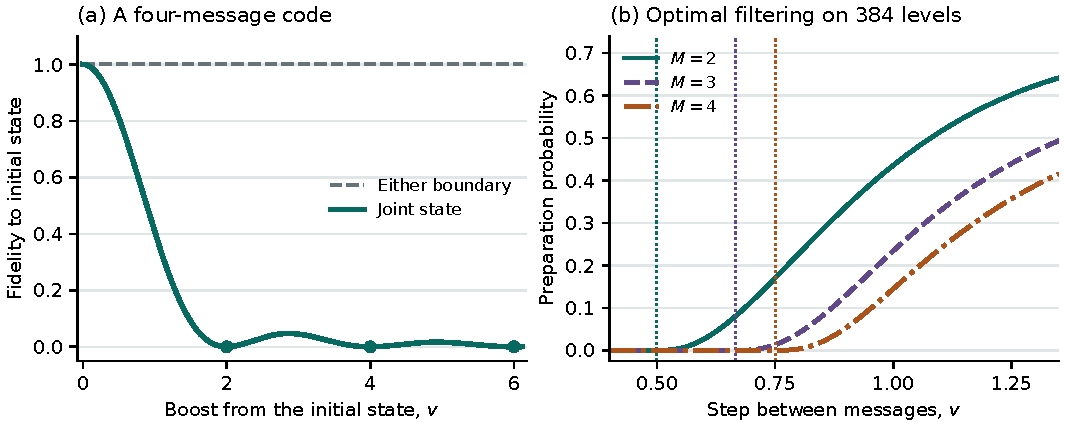
\includegraphics[width=\linewidth]{figures/boosts.pdf}
\caption{The left panel shows the squared joint overlap from \eqref{eq:sinc} and the fidelity of either marginal. The marked displacements, together with zero, form four mutually orthogonal messages in the limit. The right panel gives the optimal success at each step for the constructed 384-level distribution of Sec.~\ref{sec:numerics}. Vertical lines mark $1-1/M$.}
\label{fig:boost}
\end{figure}

\section{The optimal success probability for one bit}
For $M=2$, the limiting admissibility condition reduces to cancellation of one complex integral. Write $t=2\pi v$, $\eta_c=2\pi^2/\sg$, and $\epsilon=1-\eta_c/\eta=1-\pi/t$. The continuum problem for $t>\pi$ is
\begin{equation}\label{eq:primal}
 \Prob(t)=\sup_{0\leq h\leq1}
 \left\{\int_0^1 h f\,\dd x\ \bigg|\ \int_0^1 h(x)f(x)e^{itx}\dd x=0\right\}.
\end{equation}
A common filter is chosen before the bit. We first take the large-area limit at fixed $t$, and then let $t$ decrease to $\pi$.

\begin{theorem}\label{th:power}
For $f(x)=p x^{p-1}$ with $p>1$, the optimal filter sufficiently close to threshold accepts $[0,a]\cup[1-b,1]$. Its widths and success probability obey
\begin{align}
 a&\sim A_0\epsilon,\qquad b\sim A_0^p\epsilon^p/p,\qquad A_0=(p+1)/p,\label{eq:width}\\
 \Prob(t)&=2 A_0^p\,\epsilon^p[1+o(1)]. \label{eq:power}
\end{align}
For each fixed $t$ in this neighborhood, the optimal finite-diamond probability converges to \eqref{eq:primal}.
\end{theorem}
\begin{proof}
On the upper interval put $y=1-x$. Since $t=\pi+t\epsilon$, cancellation for the two intervals is equivalent to
\begin{equation}\label{eq:balance}
 \int_0^a p x^{p-1}e^{itx}\dd x
 =e^{it\epsilon}\int_0^b p(1-y)^{p-1}e^{-ity}\dd y .
\end{equation}
Substitute $a=A\epsilon$ and $b=B\epsilon^p$. Divide the real part of the difference by $\epsilon^p$ and the imaginary part by $t\epsilon^{p+1}$. The two limiting equations are
\[
 A^p-pB=0,\qquad \frac{p}{p+1}A^{p+1}-pB=0 .
\]
The positive solution has $A=A_0$ and $B=A_0^p/p$. The Jacobian determinant there is $p^2 A^{p-1}(A-1)>0$. Rescaling each integral to $[0,1]$ gives continuous extensions in $\epsilon\geq0$ with continuous first derivatives in $(A,B)$ near this solution. For the imaginary parts this follows from continuity of $\sin z/z$ at zero. The implicit function theorem with parameter supplies exact endpoints for all sufficiently small positive $\epsilon$, giving \eqref{eq:width}.

A dual bound proves global optimality. Let
\[
 \phi=\tfrac12 t(a+1-b),\qquad d=\tfrac12t(1-b-a),\qquad
 g(x)=1-\frac{\cos(tx-\phi)}{\cos d}.
\]
Since $A_0>1$, $0<d<\pi/2$ near threshold. Both distances from $\phi$ to $0$ and to $t$ are less than $\pi$. Thus $g$ is positive on the interiors of the two accepted tails and negative between them. For every feasible $h$, the complex constraint in \eqref{eq:primal} yields
\[
 \int h f\,\dd x=\int h g f\,\dd x\leq\int \max(g,0) f\,\dd x.
\]
The endpoint filter saturates this bound. Its mass is $a^p+1-(1-b)^p$, giving \eqref{eq:power} with a contribution of $A_0^p\epsilon^p$ from each end.

Finally, any weak limit of the finite accepted subprobabilities $h_D\mu_D$ is dominated by $\mu$ and obeys the limiting moment constraint. Its mass is at most $\Prob(t)$. Lemma~\ref{lem:correct} applied to the two intervals gives the matching lower bound. This argument requires only weak convergence at each fixed $t$.
\end{proof}

The exponent in \eqref{eq:power} has a direct gravitational origin within the assumed ensemble. At threshold, the lowest and highest area phases must be antipodal. Just above threshold the low-area tail contains only $a^p$ of the mass, while a much narrower high-area interval already supplies its counterpart. For the one-loop value of $p$, reducing $\epsilon$ by a factor of ten asymptotically reduces the best preparation probability by a factor of $717.06$.

\begin{figure}[htbp]
\centering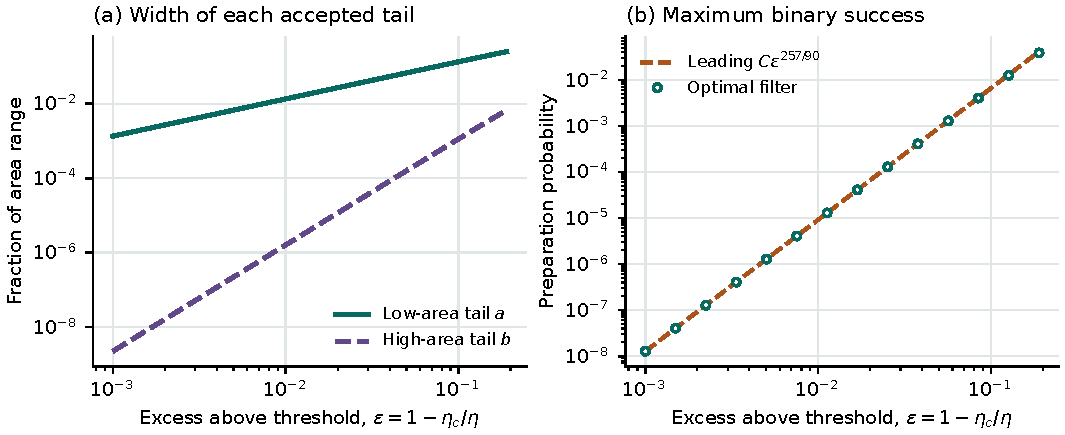
\includegraphics[width=\linewidth]{figures/threshold.pdf}
\caption{The optimal binary filter near threshold. The left panel shows the two accepted widths from \eqref{eq:balance}. The right panel compares the success probability at those endpoints with the asymptote \eqref{eq:power}, where $C=2[(p+1)/p]^p$. Both panels use logarithmic axes.}
\label{fig:optimum}
\end{figure}

\section{Reading out the relative frame}
There is an explicit one-way local decoder for any exactly orthogonal alphabet in \eqref{eq:moments}. Label the $d$ occupied Schmidt basis vectors $j=0,\ldots,d-1$, counting all degeneracies. The left boundary measures in the discrete Fourier basis of these vectors. Each outcome $r$ has probability $1/d$ for every message. After receiving the classical value of $r$, the right boundary has conditional state
\[
 |\chi_{m,r}\rangle_R=\sum_j\sqrt{w_j}\,
       e^{2\pi i m v x_j-2\pi i rj/d}|j^*\rangle .
\]
Its overlap with $|\chi_{n,r}\rangle$ is exactly \eqref{eq:moments}. A projective measurement depending on $r$ therefore recovers $m$ in one shot. For two pure states, local distinguishability with classical communication is a general result~\cite{walgate}. The Fourier-basis construction here covers every finite alphabet of this form. Its operational assumption is access to the full two boundary algebras, including coherent measurements across area sectors.

One can bound the resources of a readout interacting with a label-independent ancilla. Extend $S=\hat s_R$ by the identity on the left and on the ancilla. Suppose an interaction $H(u)$ implements a unitary $V$ in time $T$, followed by a pointer effect $0\leq F\leq1$ commuting with $S$. Take the integral below to be finite. In operator norm, Duhamel's formula and the product rule give
\begin{equation}\label{eq:cost}
 \lVert[S,V]\rVert\leq {\cal R},\qquad
 {\cal R}=\hbar^{-1}\int_0^T\lVert[S,H(u)]\rVert\dd u,\qquad
 \lVert[S,V^\dagger FV]\rVert\leq2{\cal R}.
\end{equation}
If the pointer discriminates neighboring messages with equal-prior error $e\leq1/2$, their detection probabilities differ by at least $1-2e$ for a binary decision effect. Integrating the boost derivative of that effect bounds the difference by $|\eta|\lVert[S,V^\dagger F V]\rVert/(2\pi)$. Consequently $\mathcal R\geq\pi(1-2e)/|\eta|$. Perfect readout at the step of the four-message example requires $\mathcal R\geq\sg/(8\pi)$. A time bound follows if the apparatus has a specified upper bound on $\lVert[S,H]\rVert/\hbar$.

The spectral width is essential to the protocol. For input supported on a dimensionless area band of width $w$, a common area offset cancels and the arc argument uses $|\eta|w$ in place of $|\eta|\sg$. A preparation with $w=o(\sg)$ cannot achieve the same discrimination at a step of order $1/\sg$. Determining which gravitational sources can implement the decoder, and with what time and energy budget, remains an open physical question.

\section{Numerical checks}\label{sec:numerics}
A finite model makes the distinction between the area distribution and the underlying levels explicit. For $j=1,\ldots,J$ set
\begin{equation}\label{eq:toy}
 s_j=j\log2,\qquad \sg=J\log2,\qquad
 g_j=2^j\big(\lfloor j^p\rfloor-\lfloor(j-1)^p\rfloor\big).
\end{equation}
The integer $g_j$ is a multiplicity. The cumulative thermal weight below $X=x$ is $\lfloor\lfloor Jx\rfloor^p\rfloor/\lfloor J^p\rfloor$, which tends to $x^p$. This is a constructed control for the assumed law. The Python verifier computes the floors using integer powers and uses floating point for the calibration and linear programs.

\begin{table}[htbp]
\centering\small
\begin{tabular}{rccc}
\toprule
Levels $J$ & Calibrated success & Initial $\max_{m\ne n}|G_{mn}|$ & Calibrated $\max|G-I|$\\
\midrule
32  & 0.31171 & 0.05849 & $<10^{-15}$\\
128 & 0.36507 & 0.01535 & $<10^{-15}$\\
512 & 0.38625 & 0.00388 & $<10^{-15}$\\
\bottomrule
\end{tabular}
\caption{Four messages at $v=2$ in the finite model \eqref{eq:toy}. Initial overlaps use \eqref{eq:uniform}. The correction \eqref{eq:repair} enforces their cancellation. The last column gives observed double-precision residuals.}
\label{tab:finite}
\end{table}

For Fig.~\ref{fig:boost} the linear program maximizes $\sum_j y_j$ over accepted masses $0\leq y_j\leq\mu_j$, subject to the real and imaginary parts of all $M-1$ moment constraints. For Fig.~\ref{fig:optimum} we solve the two scaled equations \eqref{eq:balance} by quadrature. This gives optimal probabilities $0.0002107906$ at $\epsilon=0.03$ and $0.0000091656$ at $\epsilon=0.01$. A separate linear program with 2,304 cells, concentrated near both endpoints and weighted by their exact continuum law, agrees with the continuum optimum to relative error below $10^{-5}$ at $\epsilon=0.06$ and $0.10$. The repository includes the script, both vector figures, and build instructions.

\section{Discussion}
A change of relative frame of order $1/\sg$ can encode information visible in correlations alone. The phase range fixes the minimal step for each alphabet. The preparation rate near that step records the low-area probability of the input ensemble. Reporting both quantities distinguishes a geometric ability to accumulate opposite phases from a probability of preparing them. Equations~\eqref{eq:power} and \eqref{eq:cost} give separate scales for preparing an accepted pair and for extracting its message. Testing these results directly in a finite-diamond calculation requires the accessible two-boundary state and control of its area coherence.

\appendix
\section{Replica moments and a zero of the gluing amplitude}
For the unfiltered state $\rho_D$ assume also $\log Z_1=o(\sg)$, as in Eqs.~(5.58) and (5.65) of Ref.~\cite{chandra}. The exact identity
\[
 \Tr\rho_D^n=Z_1^{1-n}\E_{\mu_D}\exp[-(n-1)\sg X]
\]
determines the leading R\'enyi entropies $S_n=\log\Tr\rho_D^n/(1-n)$. For fixed $0<n<1$, the exponential rate of the expectation follows by restricting to $X\geq1-\delta$ and then sending $\delta\downarrow0$. For $n>1$ use $X\leq\delta$. Both intervals have positive limiting mass. At $n=1$ one takes the mean of $X$. This gives
\begin{equation}
 \lim_{D}\frac{S_n}{\sg}=
 \begin{cases}
 1,&0<n<1,\\
 p/(p+1)=257/347,&n=1,\\
 0,&n>1 .
 \end{cases}
\end{equation}
The order of limits matters for a fluctuating-area preparation. Related work on fixed-area states analyzes the leading flattening of holographic entanglement spectra~\cite{dong}.

In the window $n=1+z/\sg$, set $\Phi_D(z)=\E_{\mu_D}e^{-zX}$. Bounded support and moment convergence give locally uniform convergence of its power series to
\begin{equation}
 \Phi(z)=p\int_0^1 x^{p-1}e^{-zx}\dd x
     =\sum_{k\geq0}\frac{p}{p+k}\frac{(-z)^k}{k!}.
\end{equation}
For real $z$, $S_{1+z/\sg}/\sg\to-\log\Phi(z)/z$, continued at zero. The variance of $-\log\rho_D$ divided by $\sg^2$ tends to $p/[(p+1)^2(p+2)]=0.0395619560\ldots$.

There is a simple zero $z_0\simeq3.597297933+8.246608718i$. The verifier bounds $\Phi$ and $\Phi'$ at the rational center $3.597298+8.246609i$ using 71 exact Taylor terms. For each series the tail is bounded by $2\cdot10^{71}/71!$. The resulting bounds are $|\Phi|<2.6\times10^{-9}$ and $|\Phi'|>0.0086$. On the disk of radius $10^{-6}$, $|\Phi''|\leq1$ since the real part of $z$ is positive. On its boundary the linear term dominates the constant and the quadratic remainder. Rouch\'e's theorem puts exactly one zero in the disk, counting multiplicity. By locally uniform convergence a finite-system zero converges to it. Reality of the density gives the conjugate zero as well.

Choose $a=\Re z_0$ and $\eta\sg=2\pi|\Im z_0|\simeq51.81497$. The monotone acceptance $h(x)=e^{-ax}$ gives success tending to $\Phi(a)\simeq0.09417834$. The normalized gluing amplitude tends to
\[
 \frac{\Tr(\rho_D e^{-aX}U_R(\eta))}{\Tr(\rho_D e^{-aX})}
 \ \longrightarrow\
 \frac{\Phi(a-i\eta\sg/(2\pi))}{\Phi(a)}=0 ,
\]
where the trace is over the area-carrying factor. Tuning to its finite-system zero makes the binary overlap exactly zero. The success operator $e^{-aX/2}$ equals an additional imaginary corner rapidity $i\pi a/\sg$ in the preparation. For the unfiltered limiting law, integration by parts gives $\Phi(-it)=0$ only if $e^{it}=\int_0^1(p-1)x^{p-2}e^{itx}\dd x$ for $t\ne0$. The right side is a strict convex average of distinct phases and has modulus below one. This explains why the tilt enters this finite-scaled-rapidity construction.

\section{A local test of arithmetic area spacing}
An additional probe uses the two-sided shear correlator of a \emph{smooth-corner} preparation in Eqs.~(5.26)--(5.29) of Ref.~\cite{chandra}. If all participating areas in units of $4G_N\hbar$ lie on $s_0+\Delta s\,\mathbb Z$, the boost at $\eta=4\pi^2/\Delta s$ acts by a common phase and restores the correlator exactly. The normalized semiclassical correlator is $\operatorname{sech}^2(\eta/2)$ to leading order. At $\Delta s=2\pi$ the lattice predicts unity at the return. The smooth-corner value at the same rapidity is $0.00744195$. The scale hierarchy must remain controlled at that particular boost, including the support and width of the boosted shear insertion as in Eq.~(D.27) of the source. Relating such a corner spectrum to stationary black-hole spectroscopy~\cite{bekenstein} would require an identification of the relevant area sectors. The coarse distribution \eqref{eq:law} by itself leaves those spacings undetermined.

\paragraph{Research materials.}
The \href{https://github.com/rkka02/pioneer/tree/main/physics/corner-boost-information}{Pioneer project folder} contains the editable manuscript and its numerical verifier. This research manuscript and the accompanying calculations were developed with assistance from OpenAI Codex.

\begin{thebibliography}{9}
\bibitem{chandra}
V.~Chandrasekaran, \emph{An algebraic quantization of gravity from the null cone},
\href{https://arxiv.org/abs/2611.34924v1}{arXiv:2611.34924v1} (2026).
\bibitem{bianchi}
E.~Bianchi and W.~Wieland, \emph{Horizon energy as the boost boundary term in general relativity and loop gravity},
\href{https://arxiv.org/abs/1205.5325}{arXiv:1205.5325} (2012).
\bibitem{margolus}
N.~Margolus, \emph{The maximum distinctness of physical systems},
\href{https://arxiv.org/abs/2111.00297}{arXiv:2111.00297}, version 4 (2025).
\bibitem{walgate}
J.~Walgate, A.~J.~Short, L.~Hardy, and V.~Vedral, \emph{Local distinguishability of multipartite orthogonal quantum states},
Phys.\ Rev.\ Lett.\ \textbf{85}, 4972 (2000).
\href{https://arxiv.org/abs/quant-ph/0007098}{arXiv:quant-ph/0007098}.
\bibitem{dong}
X.~Dong, D.~Harlow, and D.~Marolf, \emph{Flat entanglement spectra in fixed-area states of quantum gravity},
JHEP \textbf{10}, 240 (2019).
\href{https://arxiv.org/abs/1811.05382}{arXiv:1811.05382}.
\bibitem{bekenstein}
J.~D.~Bekenstein and V.~F.~Mukhanov, \emph{Spectroscopy of the quantum black hole},
Phys.\ Lett.\ B \textbf{360}, 7--12 (1995).
\href{https://arxiv.org/abs/gr-qc/9505012}{arXiv:gr-qc/9505012}.
\end{thebibliography}
\end{document}
